% \documentclass[a4paper,10pt]{article}
% \usepackage[utf8]{inputenc}
% \usepackage[pdftex]{graphicx}

\documentclass[conference]{IEEEtran}

% %\usepackage{todonotes}
\usepackage{amsmath}
\usepackage[pdftex]{graphicx}
\usepackage{epstopdf}
%\usepackage[caption=false,font=normalsize,labelfont=sf,textfont=sf]{subfig}
\usepackage{soul}
\usepackage[tight,footnotesize]{subfigure}
\usepackage{url}


% correct bad hyphenation here
\hyphenation{op-tical net-works semi-conduc-tor}

% Title Page
\title{On the Integration of Heterogeneous Data Sources for the Collaborative Internet of Things}
\author{\IEEEauthorblockN{Federico Montori, Luca Bedogni, Luciano Bononi
\IEEEauthorblockA{
Department of Computer Science and Engineering (DISI)\\
University of Bologna, Italy\\
Email: \{federico.montori2, luca.bedogni4, luciano.bononi\}@unibo.it}}
}


\begin{document}
\maketitle

\begin{abstract}
The Internet of things is foreseen as one of the next imminent Internet revolutions, as many devices will seamlessly communicate together to provide new and exciting services to the end users. One of the challenges that the IoT has to face is about both the heterogeneity of the available data and the heterogeneity of the communication. In this paper we focus on the former, by presenting an architecture able to integrate data coming from different sources, including custom made deployments and governmental data, and deliver new services made by the end users.

\end{abstract}

\section{Introduction}
Internet of Things (IoT) is one of the research and industrial fields that faced a rapid growth in the recent years.
The approach to such ecosystem has been heterogeneous and sparse, leading to a wide variety of standards and solutions at each layer of the network and application stack.
It has been a source of interest from many different points of view, in such a way that now we have dedicated infrastructures at physical, data link, network, transport and application layers.
\\

Since the beginning of its diffusion, its potential has been explored in various fields of application and its major usefulness has been claimed to be in service composition and interoperability \cite{atzori2010internet}.

The requirements when designing collaborative IoT-related automation systems are varying due to the heterogeneity of the platforms and the hardware components as well as the network interfaces.
This resulted in a sparse set of technologies and terminologies used in several scenarios determining a lack of interoperability among systems.
The common approach to the problem of unifying entities within an ecosystem is typically architectural and leads to a difficult reuse of the components among different solutions \cite{krco2014designing}.
To face these issues the European Commission supported initiatives like IoT-A \cite{iot-a}, which aimed to release an architectural reference model and FI-WARE \cite{fiware}, which also helped architects in establishing an unified vision and nomenclature and now had become an implementation-driven open community.
It also provided a sandbox in which partners could upload their open data, however it is not of broad use nowadays.
However, such solutions did not solve the problem introduced by architectures, in fact different solutions tend to create separate islands which are hard to unify.
\\

In this paper we aim to show the usefulness and the potential of open data exploitation for global cooperative IoT automation scenarios.
As a preliminary approach, we focused our analyses on data coming from two of the main open data platforms for sensors: ThingSpeak and SparkFun.
Such platforms can be queried for data streams, supplied with a set of metadata, which gave us the motivation for such proposal.
In fact, raw data streams come with temporal information, especially regarding the stream creation date and last update date.
Such parameters can tell us much about the general trend in the usage of these platforms throughout a time window of few years.
Each stream in ThingSpeak comes with a creation date, which we reported, after a data extraction, in the diagram in figure~\ref{creationtrend}.
\begin{figure}[!b]
\centering
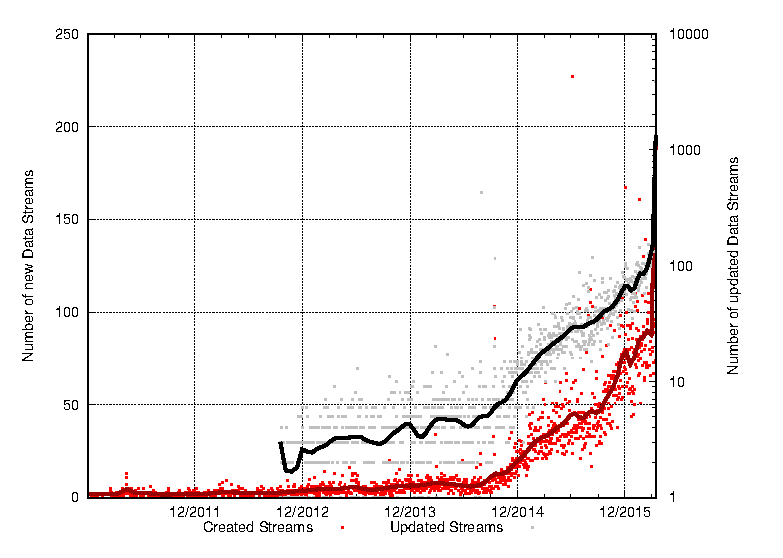
\includegraphics[width=0.50\textwidth]{img/bars.eps} 
\caption{Trend in creation of ThingSpeak channels.}
\label{creationtrend}
\end{figure}
Starting from such analysis it results a substantial growth in created channels.
Some of the steeper slopes are probably justifiable.
A possible intuition behind them is the parallel innovation in simple hardware modules, for instance August 2014 corresponds to the launch of the first version of ESP8266 \cite{esp8266} on the market and in October 2014 was possible to flash its firmware though an SDK \cite{espressif}.
Such period has not surprisingly been affected by a rapid growth according to the diagram. [TODO MORE EXAMPLES]
The diagram reports also the last update date for each stream.
It is immediately clear that, since the oldest update date is in September 2012 while the oldest creation date is in 2010, all the data streams created before 2012 that did not perform an update after such date have been deleted due to a certain policy.
The steepness of the curve in the last days reveals that a significant amount of the data streams are still in use and updated daily or even hourly.
\\

Such analyses shed some light on how rapidly the world of open data is growing and people are gaining interest in using a platform that takes away the burden of creating a local ecosystem.
Thus, our work creates the basis for a solid global ecosystem with a strong impact on cooperative services.

\section{Related Work}
% motivation: perchè fare questo? Il nostro framework porta il vantaggio dell'utilizzo degli open data e dei dati di cui c'è chi non può disporre per mancanza di materie prime (hardware) ed è possibile comporre i propri servizi grazie a un orchestratore (che banalmente mi trova il dato che mi serve senza che io debba per forza sapere id, cazzi e mazzi ecc...)
% moltissimi sono i casi in cui le architetture custom propongono la loro soluzione iot based, ma questo porta a una massiccia creazione di isole indipendenti, dove le soluzioni sono spesso incompatibili tra loro (supercazzola sulle varie soluzioni sia cloud- based sia distribuite, si può parlare di alljoyn, cumulocity, xively, iotivity, thread, nimbits ..... )
% vedi: A Survey of Commercial Frameworks for the Internet of Things (che peraltro è dei tizi di Arrowhead) 
% un altro bel repo da cui attingere è http://www.datamation.com/open-source/35-open-source-tools-for-the-internet-of-things-3.html ( questo invece parla degli open source)

The IoT is nowadays growing exponentially together with the number of solutions and architectures proposed to handle it.
The total number of connected devices is expected to be 27 billions by 2024, while the total revenue opportunity is predicted to be up to \$1.6 trillions \cite{machina} .

Regardless of the different perspectives, it is clear that the number of devices is growing, the data is becoming more and more heterogeneous, and one of the main challenges is how to handle such an amount of data and how to give a meaning to it.
In the recent years there have been a huge number of attempts which, most of the times, are either self-contained since they require compliance to a specific framework, or commercial solutions.
\\

% [SOLUZIONI DI RICERCA][...]
% \\

% [SOLUZIONI COMMERCIALI]
Commercial solutions aim to constitute a living ecosystem in which entities are ``plugged'' and interoperable, participating for the benefit of the whole system and fully compliant with the other actors within the environment.
Most of the times such frameworks, some of them depicted in \cite{derhamy2015survey}, provide efficient software adapters for legacy systems.
Such types of frameworks are often self contained and tend to create a cluster of devices which need to be framework-compatible in order to interoperate.
An example is Cumulocity \cite{cumulocity}, a platform providing an unified service oriented HTTP REST interface to devices.
Another project gaining interest in recent years is AllJoyn \cite{alljoyn}, developed by the Allseen Alliance.
Such a framework again forces devices to either implement an attachment to a software bus between application, which is indeed the AllJoyn core, or connect to an AllJoyn router using a thin library.
Either way, the communication introduces very low overhead and grants access to even constrained device.
However, the protocol used is highly customized and makes AllJoyn a quite isolated ecosystem.
Another example is Xively \cite{xively}, which, again, allows devices to obtain interoperability even among different application protocols (CoAP, MQTT, HTTP, XMPP and others) offering an API that implements a custom message bus.
Finally, another ecosystem to mention is the one implemented by Open Mobile Alliance, named OMA-LwM2M \cite{omalwm2m}, which defines a custom layer over CoAP focused on exchanging instances called ``objects'' and operating upon them via the custom interfaces.

\section{Open data as a source}
\label{sec:open}
% noi diciamo: esistono già degli open data (più o meno open). Perchè non accomunarli in un unico framework dal quale accedervi?
% Thingspeak, sparkfun (ne abbiamo presi 2 dei più popolari, e spariamo il grafico con qualche stats)

As stated in the introduction, open data are the most powerful source of information when such data are not producible by the utilizers themselves.
In this section we outline two well-known sources that we considered in order to achieve an homogeneous data store.
From both sources we extracted open data in the form of data streams (or, similarly, data channels), locations relative to one user each in which such user uploads measurements produced by its sensors.

\subsection{ThingSpeak}
ThingSpeak \cite{thingspeak}, originally launched in 2010 by ioBridge, is an open source data platform and API for the IoT that allows the user to collect, store and analyze data.
In more detail, it provides a personal cloud that users can deploy over their Local Area Network and easily display the data produced by sensors using ThingSpeak's straightforward API.
Data analysis and visualization have been made possible due to the close relationship between ThingSpeak and Mathworks, Inc. since such functionalities are driven by the integrated MatLab support. 

Furthermore, such a platform provides a global cloud hosting millions of open data records, called channels, which is useful both to users who cannot deploy their own cloud and to consumers who need to infer information coming from the stored data.
Data is stored with an absolute freedom of expression, meaning that any data channel can have any name and does not need to stick to any format constraint.
Data channels can be both private and public and provide also raw measurements encoded in XML, JSON or CSV and can be updated with new measurements every 15 seconds, according to the ThingSpeak documentation page.

In the recent years, ThingSpeak had become very popular due to the rise of easily programmable IoT platforms such as Arduino \cite{arduino}, BeagleBone Black \cite{bbblack}, ESP8266 \cite{esp8266} and many others.
Such devices are becoming cheaper and cheaper and, on the other hand, it is easier to get started with them.
Nowadays, for instance, an ESP8266 is able to manage a sensor, get connected through WiFi, be programmed through the simple, C-like Arduino SDK and still cost less than 5\$ while its battery, if the duty cycle is light enough, is estimated to have a duration of around 7 years \cite{di2015design}.
With a WiFi connection and an open platform such as ThingSpeak, a first home sensor network is very easy to bootstrap, since the device owner does not need to have the control on the cloud and, furthermore, the data produced by the sensor is easily displayable on the end consumer's personal device, such as a Smartphone or similar.

\subsection{Sparkfun}
SparkFun Electronics, Inc. \cite{sparkfun}, founded in 2003 in Colorado, is a microcontroller seller and manufacturer, known for releasing all the circuits and products as open-source hardware.
Along with the latter, it also provides tutorials, examples and classes.

For the purpose of the present paper, SparkFun also hosts its own open source cloud of open data\footnote{\url{https://data.sparkfun.com/}}, on which the customers can test and upload the data collected by the embedded sensors. %\cite{sparkfundata}
Users can push for free their data on such cloud in streams of 50 MB maximum size and with a maximum frequency of 100 pushes every 15 minutes.
Unlike ThingSpeak, the location where the data comes from is specified at a coarse granularity since the name of the city is often obtainable, however the real GPS coordinates are never given.
On the other hand, data coming from SparkFun cannot be private and consumers can download stream contents encoded in JSON, XML, CSV, MySQL, Atom and PostgreSQL.

\section{Data Unification}
\label{unification}
In this section we point out the data streams' characteristics obtainable from our two open data clouds and how do we aim to unify them onto a single data cloud.
We extracted the whole repositories and parsed the JSON files in order to give a first structure to such data.
Since the data structure does not force strong constraints data is, as explained in detail in section~\ref{unification}, often incomplete.

Hereby are briefly presented the parameters that can be extracted from data streams:
\begin{itemize}
 \item \textbf{Stream ID}: it is the data stream's unique identifier. In ThingSpeak it is represented by an incremental number, which is assigned when the stream is created. At the time of writing there are 28806 active streams with IDs spanning from 1 to 100172. In SparkFun the unique ID is given by a string of 20 random ASCII characters. At the time of writing we counted 3575 different SparkFun IDs. 
 \item \textbf{Stream name}: it present in both platforms and it is decided by the user with no constraint. This means that it can even carry no useful information for its identification and categorization.
 \item \textbf{Geolocalization}: it is present in both platforms. In ThingSpeak not all the streams come with geolocalization data, however it is always given in GPS coordinates. Similarly, in SparkFun not all the streams are geolocalized, however, when they are, no GPS coordinates are given, but only the name of the city, or sometimes just the state or even the country, unless the user indicates the GPS coordinates in the data itself.
 \item \textbf{Tags}: are included in both platforms and often help to infer useful information about the data.
 \item \textbf{Creation Timestamp}: it is included in all ThingSpeak streams as a metadata, on the other hand, the creation date of a SparkFun stream is not included. Each SparkFun stream is limited to 50 MB, thus the first update of any SparkFun stream smaller than 50 MB corresponds to its creation date,  however it is retrievable in a limited number of cases.
 \item \textbf{Last Update Timestamp}: it is included in all ThingSpeak streams as a metadata. In SparkFun is simply deducible from the timestamp of the last update in the stream, since the timestamp is included in each data update.
 \item \textbf{Description}: it is a ThingSpeak metadata and its characterization is fully assigned to the user (who can also decide not to include it).
 \item \textbf{Elevation}: it is a ThingSpeak metadata and not always indicated.
 \item \textbf{Last Entry ID}: it is a ThingSpeak metadata, which points to the last update record in the data, ordered using an incremental ID for each update.
\end{itemize}

From each data stream we extracted in particular the GPS position for a locational analysis, finding that such position is indicated, with different degree of precision, in 6665 data streams out of 32381.
In 32\% of such cases, only a macro area is given (the city, or even the state).
These are the cases coming from SparkFun, for which we took the central position of the indicated entity using the Google Maps API.
The result of the analysis is outlined in figure~\ref{geo}.

\begin{figure*}[!t]
\centering
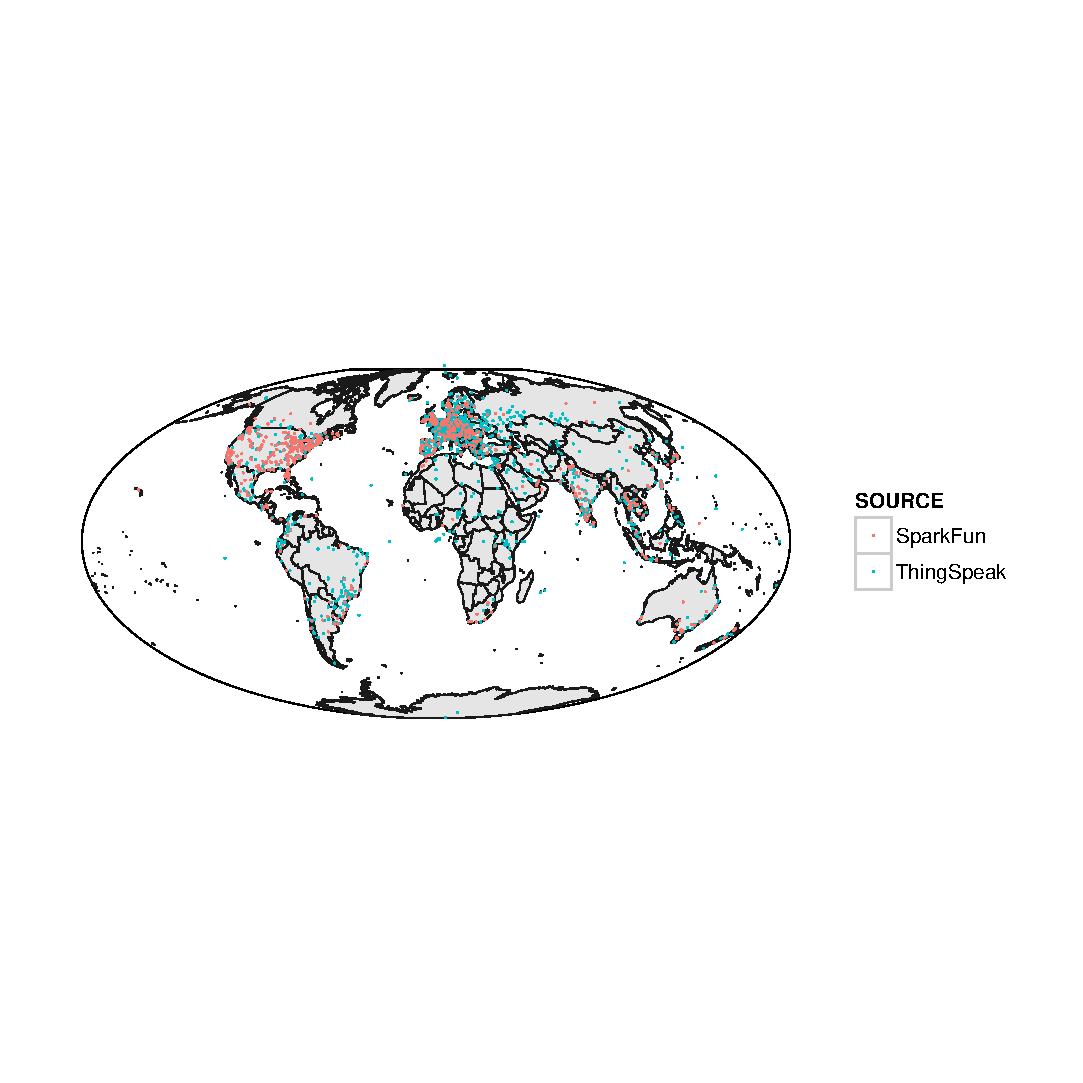
\includegraphics[width=1\textwidth]{img/map.eps} 
\caption{Location of all ThingSpeak and SparkFun sensing sources.}
\label{geo}
\end{figure*}

Given such results, the importance of information fusion from different sources is clear, since not only the sampling number of the sensing infrastructure is incremented, but also its coverage.
Indeed, ThingSpeak appears to have much more utilization in the European region, whereas SparkFun seems to be more popular in North America.
Furthermore, this consideration might be extended to different macro topic areas, meaning that some open data sources are specialized on a specific field of measuring.
For instance, governmental sources providing open data such as EPA (United States Environmental Protection Agency) \cite{epa} are primarily focused on environmental data, whilst crowdsensing sources such as OpenSignal \cite{opensignal} regard measurements on cellular network signal strength and coverage.
\\

Therefore, a basic unification counting on an essential set of metadata is crucial, composing the minimum skeleton to which a data stream should be linked.
For such purpose we aim to design an unique ID assignment policy, a geolocalization (with a precision error), a freshness of the information (given by the last update timestamp), a friendly name and an inferred measurement category (such as temperature, humidity and so on) together with an unit of measure.

%[TODO FEEDBACK]

\section{Our Architectural Proposal}
\label{sec:casestudy}
In this section we discuss the our proposal and how we intend to carry out the architectural design.
We also give a glimpse on the case studies for this scenario in order to show why would someone use open data integration for measurement tasks.
\\
Figure~\ref{arch} shows an architecture depicting several use cases.

\begin{figure*}[!t]
\centering
\includegraphics[width=1\textwidth]{img/Archit.eps} 
\caption{}
\label{arch}
\end{figure*}

In our proposed architecture we assume to have a decision middleware, called Orchestrator, which is capable to return a service record, or a data stream, given a set of parameters determined by the user's choice.
Such information is returned from one among the sources available, provided that the user specified his or her preference for ``reliable'' or ``unreliable'' data, which namely corresponds to official or user-defined respectively.
We also aim to have our own data cloud for both data streams and services which are not intended to be published as open data onto one of the sources mentioned.

As a case study, an user can run an application making use of different measurements, for instance outdoor temperature and the amount of fine dust or pollen in the air, in order to infer an environmental condition or to trigger some action.
For instance it would open automatically the window that is not facing the sun when it's too hot, but just if the pollen in the air is below a certain threshold, otherwise it turns on the air conditioning in order to avoid allergic reactions.
Such a case study could happen in several situations.
An user, for example, might be the owner of the temperature sensor, since it is cheap and easily configurable (``Sensor 3'' in the figure).
However, other sensors such as pollen sensors or fine dust sensors might be too expensive or rare to get, or simply not owned by the end user and therefore other users' measurements are needed, provided they are nearby enough (this is also why geolocalization is meant to be crucial).

Furthermore, different data sources might have a different update rate and a different ``reliability'', since they may belong to providers that are recognized as trustworthy or not.
This happens when such providers receive several positive feedbacks due to their estimated precision and update rate.
Furthermore, in the integration presented we used two user-driven platforms, however, we aim to integrate our architecture with reliable and official data, such as EPA for the United States environmental measurements.
Such measurements, since they are official, are considered to be reliable, however their slow update rate introduces a trade-off whenever an user must choose between a high reliability or a fast update rate.
Some applications indeed might require information at a finer granularity over time, for example when they want to detect instantaneous condition changes.
In such cases the user, choosing the update frequency at the expense of reliability, will necessarily use the data or the services provided by neighbors.
\\

Our proposed architecture aims not only to unify raw data streams and make them universally available, but also to make users able to share their service endpoint and to provide additional capabilities derived from both data aggregation and personal computational capabilities (``Service 2'' in the figure).
As a simple example, an user receiving temperature and humidity data might calculate the heat index and expose it as a service interface.
\\

Our proposal, given such a various set of use cases, provides the user with a wide variety of options regarding deployment and data retrieval.
This is really important since the user is not forced to stick to a particular approach and gives a great advantage in an era where heterogeneity affects not only data and protocols, but also solutions.

\section{Conclusions}
\label{sec:conclusions}
In this paper we showed how open data express their high potential in the ecosystem of data fusion and how we aim to manage them in order to integrate heterogeneous collaborative approaches within a global vision, by exploiting heterogeneous data sources.



\bibliographystyle{IEEEtran}
% argument is your BibTeX string definitions and bibliography database(s)
\bibliography{iot}
\end{document}          
